\documentclass[a4paper]{article}
\usepackage{bbold}
\usepackage{amsmath}
\usepackage{tikz}
\title{Balancing the inverse pendulum}
\author{Norbert Braun\\\texttt{n.braun@ikp.uni-koeln.de}}
\begin{document}
\maketitle
\section{Equations of motion}
\begin{figure}
\centering

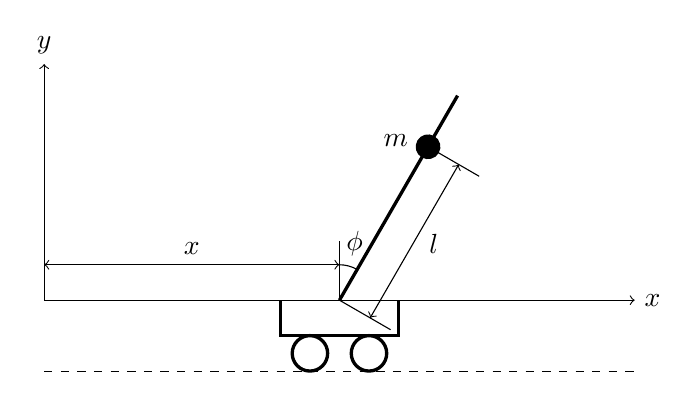
\begin{tikzpicture}[scale=1.5]
% Coordinate system
\draw[->] (0,0) -- (5,0) node[anchor=west] {$x$};
\draw[->] (0,0) -- (0,2) node[anchor=south] {$y$};

\draw[dashed] (0,-.6) -- (5,-.6);

% Cart
\begin{scope}[very thick]
    \draw (2,0) -- (2,-.3) -- (3,-.3) -- (3,0);
    \draw (2.25,-.45) circle (.15cm);
    \draw (2.75,-.45) circle (.15cm);
\end{scope}

% Pendulum
\begin{scope}[xshift=2.5cm,rotate=-30]
    \draw[very thick] (0,0) -- (0,2);
    \filldraw[fill=black] +(0,1.5) circle (.1cm);
    \draw (-.1,1.5) node[anchor=east] {$m$};
    \draw (0,0) -- (.5,0);
    \draw (0,1.5) -- (.5,1.5);
    \draw[<->] (.3,0) -- (.3,1.5);
    \draw (.35,.75) node[anchor=west] {$l$};
\end{scope}

% Helper lines
\draw (2.5,.3) arc(90:60:.3cm);
\draw (2.5,0) +(75:.5cm) node {$\phi$};
\draw (2.5,0) -- +(0,.5);
\draw[<->] (0,.3) -- (2.5,.3);
\draw (1.25,.3) node[anchor=south] {$x$};

\end{tikzpicture}

\caption{The inverse pendulum}
\label{fig:system}
\end{figure}

The system, shown in figure \ref{fig:system}, consists of a pendulum mounted on a movable cart. We choose coordinates such that the y axis is pointing up. The pendulum can rotate freely around the point at its base, but this axis is unpowered. The task will be to move the cart in such a way that the pendulum keeps pointing upwards.

For simplicity, we will assume that we can control the position $x(t)$ of the cart, rather than the force acting on it. (The latter would require taking the backreaction of the pendulum on the cart into account.) This is a rather realisitic assumption to make; a closed-loop control of the wheel velocity will realize this kind of system.

We take the position $x$ of the cart and the pendulum angle $\phi$ as generalized coordinates. We assume that the pendulum can be represented by a point mass $m$ at a distance $l$. The point mass position is given by
\begin{eqnarray}
x_p &=& x + l \sin\phi\\
y_p &=& l \cos\phi
\end{eqnarray}
resulting in a kinetic energy
\begin{equation}
T = \frac{1}{2} m v_p^2 = \frac{1}{2} m \dot{x}^2 + \dot{x}lm\dot{\phi}\cos\phi + \frac{1}{2}ml^2\dot{\phi}^2
\end{equation}
and a potential energy
\begin{equation}
V = mgl\cos\phi
\end{equation}

We will use the Lagrange function
\begin{equation}
L = T - V
\end{equation}
to get the equations of motion,
\begin{equation}
\frac{\mathrm{d}}{\mathrm{d}t}\frac{\partial L}{\partial \dot{\phi}} - \frac{\partial L}{\partial \phi} = 0
\end{equation}
In our case, we have
\begin{eqnarray}
\frac{\partial L}{\partial \dot{\phi}} &=& l m \dot{x} \cos \phi + m l^2 \dot{\phi}\\
\frac{\partial L}{\partial \phi} &=& -\dot{x} l m \dot{\phi}\sin \phi + m g l \sin \phi
\end{eqnarray}
and thus
\begin{equation}
\ddot{\phi} - \frac{g}{l}\sin \phi = - \frac{1}{l} \cos \phi \ddot{x}
\end{equation}
showing that we have to accelerate the cart to control the pendulum.

We now assume that the excursion of the pendulum from the upright position is small. Linearizing the above equation leads to
\begin{equation}
\ddot{\phi} - \frac{g}{l} \phi = - \frac{1}{l} \ddot{x}
\end{equation}

\section{Stabilizing the pendulum}
To actually stabilize the pendulum, we will use a linear function
\begin{equation}
\ddot{x} = a(t) = a_1 \dot{x} + a_2 \dot{\phi} + a_3 x + a_4 \phi
\end{equation}
The reason to include $x$ in the function is that, without it, the cart would accelerate to correct a deviation in the pendulum position, but then not have a reason to stop and eventually hit the wall. By including the cart position in the function, we can control it together with the pendulum angle.

The equations of motion of the system thus become
\begin{eqnarray}
\ddot{\phi} &=& \frac{g}{l} - \frac{1}{l} a(t)\\
\ddot{x} &=& a(t)
\end{eqnarray}

In matrix form, these can be written as
\begin{equation}
\label{eqn:matrixform}
\frac{\mathrm{d}}{\mathrm{d}t}\left(\begin{array}{l}
\dot{x}\\ \dot{\phi}\\ x\\ \phi \end{array}\right)
= \left(\begin{array}{cccc}
a_1 & a_2 & a_3 & a_4\\
-\frac{a_1}{l} & -\frac{a_2}{l} & -\frac{a_3}{l} & -\frac{a_4}{l} + \frac{g}{l}\\
1 & 0 & 0 & 0\\
0 & 1 & 0 & 0\\
\end{array}\right)
\left(\begin{array}{l}
\dot{x}\\ \dot{\phi}\\ x\\ \phi \end{array}\right)
\end{equation}
with the general solution
\begin{equation}
\left(\begin{array}{l}\dot{x}(t)\\ \dot{\phi}(t)\\ x(t)\\ \phi(t) \end{array}\right)
= \exp(A t) \left(\begin{array}{l}\dot{x}(0)\\ \dot{\phi}(0)\\ x(0)\\ \phi(0) \end{array}\right)
\end{equation}
where $A$ is the matrix from (\ref{eqn:matrixform}), and $\exp$ is the matrix exponential.

We now wish to study the eigenvalues of $A$. A tedious, but otherwise elementary calculation gives the characteristic polynomial as
\begin{equation}
\begin{split}
\xi_A(\lambda) &= \det(A - \lambda \mathbb{1})\\
&= \lambda^4 + \left(\frac{a_2}{l} - a_1\right) \lambda^3 + \left(\frac{a_4}{l} - \frac{g}{l} - a_3\right) \lambda^2 + a_1 \frac{g}{l} \lambda + a_3 \frac{g}{l}
\end{split}
\end{equation}

We want the eigenvalues of $A$ to be real and negative. In particular, let us choose all eigenvalues equal to $-k$, giving a characteristic polynomial of the form
\begin{equation}
\begin{split}
\xi_A(\lambda) &= (\lambda + k)^4\\
&= \lambda^4 + 4k\lambda + 6k^2\lambda^2 + 4 k^3\lambda + k^4
\end{split}
\end{equation}
Comparing coefficients then gives simple equations for the control parameters $a_i$:
\begin{eqnarray}
a_1 &=& 4 \frac{l}{g} k^3\\
a_2 &=& 4 k l \left(1 + \frac{l}{g} k^2\right)\\
a_3 &=& \frac{l}{g} k^4\\
a_4 &=& 6 k^2 l + g + \frac{l^2}{g} k^4\\
\end{eqnarray}

Figure \ref{fig:numeric} shows a numeric result for $k = ?$.

\section{Implementation notes}

\end{document}
